\documentclass[10pt]{article}
\usepackage{icmlko}

\icmlmeta{IP 파운데이션 월드모델}{263}{쌓이는 것을 미리 알 수는 없다}{손 축의 원본 필드를 다 훑었다 --- 웹툰 ``굿즈 규모''가 회차 수였고, 빼니 판이 올랐다}

\begin{document}

\twocolumn[
\icmlheader

\begin{abstract}
노트 262가 웹툰 ``입장 허들''이 \texttt{daily\_pass} 임을 찾고 ``나머지 넷도
훑어라''를 남겼다. 훑었다 --- 손 축 다섯 $\times$ 아홉 도메인의 원본 필드를
전부 뽑아, 쌓이는 무늬(연도 상관 · 학습 대 유보 평균비)로 걸렀다.
\textbf{하나가 더 걸렸다}: 웹툰 \texttt{goods\_scale} 이 \texttt{n\_episode}
다(노트 208이 연재 밀도에서 바꿔 놓은 것). 연도와 \textbf{$-$0.490} 이고
학습 평균 100.4 대 유보 평균 44.7(45\%)이다 --- \textbf{연재가 이어지는 동안
쌓이고, 예측 시점에는 모두가 0 이다.} 노트 208은 ``셈꼴은 시간을 담아도 해가
없다''고 적었는데 그 문장은 \emph{분모에 측정 시각이 든 비율}에 대한
것이었다. 셈꼴 자체도 쌓인다. \textbf{나머지 셋은 안 막았다}: 세계애니
\texttt{n\_episode}$\times$분은 \texttt{FINISHED} 일 때만 관측이라 연도 상관이
$-$0.063 이고, 애니 \texttt{is\_dubbed} 는 $+$0.014 로 깨끗하고, 만화
\texttt{n\_chapter} 는 \textbf{유보가 6건이라 증거 자체가 없다}(학습 113 대
유보 44 는 여섯 건의 평균이다 --- 하마터면 그 수를 근거로 쓸 뻔했다). 셋 다
막으면 판이 오히려 내려간다(0.4890 $\to$ 0.4855). 웹툰 하나만 막으니 판이
\textbf{0.4772 $\to$ 0.4842} 다. \textbf{새는 축 둘을 빼고 나서가 넣고
있을 때보다 높다}(노트 260의 0.4916 은 두 축이 새던 값이고, 지금 0.4842 는
안 새는 값이다 --- 견줄 수 있는 것은 노트 262의 0.4772 다). 가드 여덟 통과.
\end{abstract}
]

\section{다섯 축 $\times$ 아홉 도메인을 뽑았다}

노트 262가 하나를 찾고 ``\texttt{entry\_friction} 만 봤다. 넷이 더 있다''를
남겼다. 손 축 다섯의 원본 필드를 전부 뽑았다.

\begin{center}\small
\begin{tabular}{ll}
\hline
\texttt{target\_breadth} & 태그 수 · 연령 등급 · 언어 수 · 판형 \\
\texttt{venue\_prominence} & 요일 수 · 제작사 이력 · 작가 이력 \\
\texttt{entry\_friction} & 가격 · 성인 여부 · \textbf{웹툰만 \texttt{daily\_pass}} \\
\texttt{media\_push} & 스크린샷 수 · 더빙 · 퍼블리셔 \\
\texttt{goods\_scale} & 회차 수 · 용량 · 판형 · 구성 수 \\
\hline
\end{tabular}
\end{center}

쌓이는 무늬로 걸렀다 --- \textbf{연도와의 상관}과 \textbf{학습 대 유보
평균비}. 쌓이는 양은 오래된 것일수록 크므로 연도와 음의 상관이 나고, 유보
(최근)의 평균이 학습보다 작다.

\begin{figure}[t]
\centering
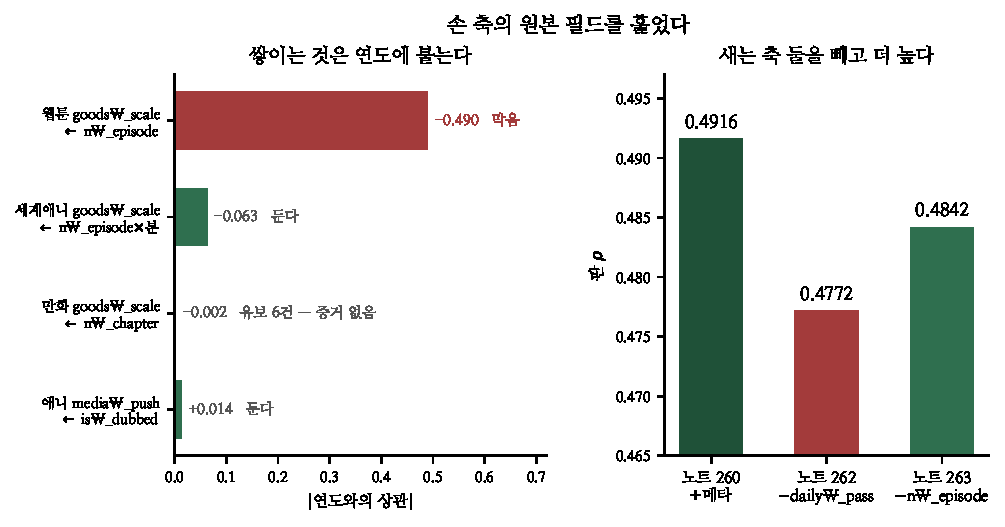
\includegraphics[width=\columnwidth]{figs/accrual.pdf}
\caption{왼쪽 --- 원본 필드의 연도 상관. 오른쪽 --- 판.}
\end{figure}

\begin{center}\small
\begin{tabular}{llrr}
\hline
도메인 · 축 & 원본 & 연도와 & 유보/학습 \\
\hline
\textbf{웹툰 \texttt{goods\_scale}} & \texttt{n\_episode} &
  $\mathbf{-0.490}$ & \textbf{45\%} \\
세계애니 \texttt{goods\_scale} & \texttt{n\_ep}$\times$분 & $-$0.063 & 81\% \\
만화 \texttt{goods\_scale} & \texttt{n\_chapter} & $-$0.002 & 39\% \\
애니 \texttt{media\_push} & \texttt{is\_dubbed} & $+$0.014 & 95\% \\
\hline
\end{tabular}
\end{center}

\section{웹툰 하나만 걸렸다}

\texttt{n\_episode} 는 연재가 이어지는 동안 쌓인다. \textbf{예측 시점 ---
연재 시작 --- 에는 모든 작품이 0 화다.} 학습 구간 작품은 평균 100화이고
유보 구간 작품은 44화인데, 그 차이는 작품의 성질이 아니라 \emph{얼마나
오래 연재했나}다.

노트 208이 이 축을 연재 밀도(회차/경과주)에서 회차 수로 바꾸면서 이렇게
적었다.

\begin{quote}\small
\textbf{비율이면서 분모에 측정 시각이 있는 축만 위험하다} --- 셈꼴은 시간을
담아도 해가 없다.
\end{quote}

\textbf{그 문장이 좁았다.} 위험한 것은 분모의 ``지금''만이 아니다 --- 셈꼴
자체가 ``지금까지''를 세고 있으면 같은 병이다. 노트 224가 웹툰 화 간격 축을
사후로 물릴 때 ``첫 스무 화는 연재 시작 후 중앙 133일 뒤에야 완성된다''고
적었는데, 회차 \emph{수}도 같은 집안이다.

\section{셋은 안 막았다}

\paragraph{세계애니} \texttt{status == FINISHED} 일 때만 관측한다(코드가
``연재중이면 사후에 늘어난다''고 이미 적어 뒀다). 연도 상관 $-$0.063, 유보/학습
81\%. 둔다.

\paragraph{애니 \texttt{is\_dubbed}} 더빙은 나중에 붙을 수 있어 의심했는데
완결과 $+$0.020 · 연도와 $+$0.014 · 유보/학습 95\% 로 무늬가 없다. 둔다.

\paragraph{만화} 학습 평균 113 대 유보 평균 44 로 웹툰보다 심해 보인다.
\textbf{그런데 만화 유보는 6건이다.} 44 는 여섯 건의 평균이고, 연도 상관은
$-$0.002 로 무늬가 없다. \textbf{하마터면 여섯 건의 평균을 근거로 축을 막을
뻔했다} --- 노트 248이 세운 규약(도메인별 수는 SE 와 함께 읽는다)이 여기서
값을 했다. 둔다.

셋을 다 막으면 판이 0.4890에서 0.4855로 \emph{내려간다}. 안 막은 것이 맞다.

\section{판}

\begin{center}\small
\begin{tabular}{lrrr}
\hline
 & F21 & F18 & \textbf{F23} \\
\hline
노트 260 (새는 축 둘 포함) & 0.4626 & 0.4875 & 0.4916 \\
노트 262 ($-$\texttt{daily\_pass}) & 0.4348 & 0.4738 & 0.4772 \\
\textbf{지금} ($-$\texttt{n\_episode}) & 0.4542 & 0.4845 & \textbf{0.4842} \\
\hline
\end{tabular}
\end{center}

\textbf{새는 축을 빼니 판이 올랐다.} 노트 260에서 \texttt{daily\_pass} 를
뺐을 때도 같았다(0.4831 $\to$ 0.4916). 두 번째다. 새는 열은 점수를
부풀리기만 하는 게 아니라 \textbf{자리를 차지해 진짜 축을 밀어낸다} ---
웹툰 \texttt{goods\_scale} 이 빠지자 웹툰이 0.4211에서 0.4418로 올랐다.

노트 260의 0.4916 과 지금의 0.4842 를 나란히 놓으면 안 된다. 앞의 것은
축 둘이 새던 값이고 지금은 안 새는 값이다. \textbf{견줄 수 있는 것은 노트
262의 0.4772 이고, 거기서 $+$0.0070 이다.}

\paragraph{남은 것}
\begin{center}\small
\begin{tabular}{ll}
\hline
갈래 & 왜 \\
\hline
채우는 쪽 시점표 & (축, 도메인) $\to$ 원본 필드를 코드에 적어 두면 \\
웹툰 손 축 셋 & 다섯 중 둘을 막았다. 남은 셋은 무엇인가 \\
천장 다시 & 두 번 막았으니 다시 재야 한다 \\
라벨 자체 & 노트 209의 누적 라벨. 축만 고치고 라벨은 그대로다 \\
\hline
\end{tabular}
\end{center}

\paragraph{규약} ``셈꼴은 안전하다''는 틀렸다. \textbf{쌓이는 것은 비율이든
셈꼴이든 사후다.} 값싼 검사는 둘이다 --- 연도와의 상관, 그리고 유보 대 학습
평균비. 다만 \textbf{그 비를 읽기 전에 유보 표본 수를 먼저 본다}(만화는
여섯 건이었다).

\end{document}
